\documentclass[addpoints]{exam}

\usepackage{amsmath}
\usepackage{amssymb}
\usepackage{enumitem}
\usepackage{graphicx}
\usepackage{hyperref}
\usepackage{multicol}
\usepackage{tikz}
\usepackage{titling}
\usetikzlibrary{positioning,chains,fit,shapes,calc}

% Header and footer.
\pagestyle{headandfoot}
\runningheadrule
\runningfootrule
\runningheader{CS 113 Spring 201}{HW 4: Functions, Induction, Graphs}{\theauthor}
\runningfooter{}{Page \thepage\ of \numpages}{}
\firstpageheader{}{}{}

\boxedpoints
\printanswers

\newcommand\union\cup
\newcommand\interx\cap

\graphicspath{{images/}}

\title{Homework 4: Functions, Induction, Graphs}
\author{associative-multiset}  % replace with your team name
\date{CS/MATH 113 Discrete Mathematics\\Habib University, Spring 2022}

\begin{document}
\maketitle

\begin{questions}

  \section*{Functions}
  
\question[5] Consider these functions from the set of students in a discrete mathematics class. Under what conditions is the
  function one-to-one if it assigns to every student,
  
  \begin{enumerate}[label=\alph*)]
  \item their mobile phone number.
    \begin{solution}
      Let S be the set of students in discrete mathematics class and let M be the set of mobile phone numbers. Then, $f: S \mapsto M$ such that every student gets assigned a mobile phone number. 
      Then, $\forall x \epsilon S \forall y \epsilon S (f(x) = f(y) \implies x = y) $. Thus, this function is one-to-one only when no two students have the same mobile phone number i.e. each student must have a unique phone number.
    \end{solution}
  \item their student identification number.
    \begin{solution}
      Let S be the set of students in discrete mathematics class and let I be the set of identification numbers. Then, $f: S \mapsto I$ such that every student gets assigned an identification number. 
      Then, $\forall x \epsilon S \forall y \epsilon S (f(x) = f(y) \implies x = y) $. Thus, this function is one-to-one only when no two students have the same identification number i.e. each student must have a unique indentification number.
    \end{solution}
  \item their final grade in the class.
    \begin{solution}
      Let S be the set of students in discrete mathematics class and let G be the set of grades. Then, $f: S \mapsto G$ such that every student gets assigned a grade. 
      Then, $\forall x \epsilon S \forall y \epsilon S (f(x) = f(y) \implies x = y) $. Thus, this function is one-to-one only when no two students have the same grade i.e. each student must have a unique grade.
    \end{solution}
  \item their home town.
    \begin{solution}
      Let S be the set of students in discrete mathematics class and let H be the set of home towns. Then, $f: S \mapsto H$ such that every student gets assigned a home town. 
      Then, $\forall x \epsilon S \forall y \epsilon S (f(x) = f(y) \implies x = y) $. Thus, this function is one-to-one only when no two students have the same home town i.e. each student must have a unique home town.
    \end{solution}
  \item their Ehsas hour appointment.
    \begin{solution}
      Let S be the set of students in discrete mathematics class and let E be the set of Ehsas hours. Then, $f: S \mapsto E$ such that every student gets assigned a Ehsas hour. 
      Then, $\forall x \epsilon S \forall y \epsilon S (f(x) = f(y) \implies x = y) $. Thus, this function is one-to-one only when no two students have the same Ehsas hour appointment i.e. each student must have a unique Ehsas hour appointment.
    \end{solution}
  \end{enumerate}


\question[5] If $f$ and $f \circ g$ are one-to-one, does it follow that $g$ is one-to-one? Justify your answer.
  \begin{solution}\\
    A function is a one-to-one if only if, for all $a$ and $b$ in domain; there exists $f(a) = f(b) \rightarrow a = b$ .\\
    \textbf{Given:}\\
    $f$ and $(f \circ g)$ are one-to-one function.\\
    \textbf{To prove:}\\
    $g$ is a one-to-one function.\\
    \textbf{Direct Proof:}\\
    Assuming,\\
    $g(a) = g(b)$\\
    Taking function $f$ on each side,\\
    $f(g(a)) = f(g(b))$\\
    By using definition of composition,\\
    $(f \circ g)(a) = (f \circ g)(b)$\\
    since, $(f \circ g)$ is a one-to-one,\\
    $a = b$\\
    Thus,\\
    $g(a) = g(b) \rightarrow a = b$.\\
    Hence,
    By the definition of one-to-one, we've proved that $g$ is a one-to-one function.
  \end{solution}

\question[5] Prove that a strictly decreasing function from $\mathbb{R}$ to itself is one-to-one. Give an example of a decreasing function from $\mathbb{R}$ to itself that is not one-to-one.
  \begin{solution}
    For a stricly decreasing function if $x < y$ then $f(x) > f(y)$.\\
    Let us assume that $f(x) = f(y)$, then:\\
    If $x < y$ then by definition of a strictly decreasing function we have that $f(x) > f(y)$, thus this is a contradiction to our assumption, thus $x \not < y$.\\
    If $x > y$ then by definition of a strictly decreasing function we have that $f(x) < f(y)$, thus this is a contradiction to our assumption, thus $x \not > y$.\\
    If $x = y$ then by definition of a strictly decreasing function we have that $f(x) = f(y)$, thus this supports our assumption, therefore we have that $\forall x \epsilon \mathbb{R} \forall y \epsilon \mathbb{R} f(x) = f(y) \implies x = y$, which is the definition of a one-to-one function, thus this function is one-to-one.\\
    An example of a decreasing function from $\mathbb{R}$ to itself can be $f(x) = -[x]$, where $[]$ denotes ceiling. This function is not one-to-one, as for example if x = 3 and y = 2.5, then $f(x) = f(y) = -3$, thus this contradicts with the definition of a one-to-one function.  
  \end{solution}
  
  \section*{Graphs}
  
\question To lift the spirits of the students on their return, Habib University has decided to build 4 new courtyards--Nature, Ice, Light, and Darkness. Designs are invited and bids are received for the courtyards from 4 architect firms as follows. Parveen Prime can design Nature, Light, and Darkness; Queen Quratulain can design Ice and Light; Reena Rani can design Light and Darkness; and Super Sonam can design Nature and Ice.
  \begin{parts}
  \part[5] Use a bipartite graph to model the four architects and the courtyards that they can design.
    \begin{solution}\\
      $V_{1}$ = \{Parveen Prime, Queen Quratulain, Reena Rani, Super Sonam\}\\
      $V_{2}$ = \{Nature, Ice, Light, Darkness\}\\
      $E$ = \{(Parveen Prime, Nature), (Parveen Prime, Light), (Parveen Prime, Darkness), (Queen Quratulain, Ice), (Queen Quratulain, Light), (Reena Rani, Light), (Reena Rani, Darkness), (Super Sonam, Nature), (Super Sonam, Ice)\}\\

      \definecolor{myblue}{RGB}{80,80,160}
      \definecolor{mygreen}{RGB}{80,160,80}

      \begin{tikzpicture}[thick,
          %every node/.style={draw,circle},
          fsnode/.style={fill=myblue},
          ssnode/.style={fill=mygreen},
          %every fit/.style={ellipse,draw,inner sep=-2pt,text width=2cm},
          ->,shorten >= 3pt,shorten <= 3pt
        ]

        the vertices of U
        \begin{scope}[start chain=going below,node distance=7mm]
          \foreach \i in {PP,QQ,RR,SS}
          \node[fsnode,on chain] (f\i) [label=left: \i] {};
        \end{scope}

        % the vertices of V
        \begin{scope}[xshift=4cm,yshift=-0.5cm,start chain=going below,node distance=7mm]
          \foreach \i in {Nature,Ice,Light,Darkness}
          \node[ssnode,on chain] (s\i) [label=right: \i] {};
        \end{scope}

        % the set U
        \node [myblue,fit=(fPP) (fSS),label=above:$A$] {};
        % the set V
        \node [mygreen,fit=(sNature) (sDarkness),label=above:$B$] {};

        % the edges
        \draw (fPP) -- (sNature);
        \draw (fPP) -- (sLight);
        \draw (fPP) -- (sDarkness);
        \draw (fQQ) -- (sIce);
        \draw (fQQ) -- (sLight);
        \draw (fRR) -- (sLight);
        \draw (fRR) -- (sDarkness);
        \draw (fSS) -- (sNature);
        \draw (fSS) -- (sIce);
      \end{tikzpicture}
    \end{solution}
    
  \part[5] Use Hall’s theorem to determine whether there is an assignment of architects to courtyards so that each architect is assigned one courtyard to design.
    \begin{solution}\\
      Assuming:\\
      P = Parveen Prime, Q = Queen Quratulain, R = Reena Rani, S = Super Sonam\\
      A = Nature, B = Ice, C = Light, D = Darkness\\
      Let us determine the neighbourhood of each subset of $V_{1}$ and check if $|N(A)| \geq |A|$ holds for all subset of $V_{1}$.\\
      $N(\emptyset) = \emptyset = 0 \geq 0$\\
      $N(\{P\}) = \{A,C,D\} = 3 \geq 1$\\
      $N(\{Q\}) = \{B,C\} = 2 \geq 1$\\
      $N(\{R\}) = \{C,D\} = 2 \geq 1$\\
      $N(\{S\}) = \{A,B\} = 2 \geq 1$\\
      $N(\{P,Q\}) = \{A,B,C,D\} = 4 \geq 2$\\
      $N(\{P,R\}) = \{A,C,D\} = 3 \geq 2$\\
      $N(\{P,S\}) = \{A,B,C,D\} = 4 \geq 2$\\
      $N(\{Q,R\}) = \{B,C,D\} = 3 \geq 2$\\
      $N(\{Q,S\}) = \{A,B,C\} = 3 \geq 2$\\
      $N(\{R,S\}) = \{A,B,C,D\} = 4 \geq 2$\\
      $N(\{P,Q,R\}) = \{A,B,C,D\} = 4 \geq 3$\\
      $N(\{P,Q,S\}) = \{A,B,C,D\} = 4 \geq 3$\\
      $N(\{P,R,S\}) = \{A,B,C,D\} = 4 \geq 3$\\
      $N(\{Q,R,S\}) = \{A,B,C,D\} = 4 \geq 3$\\
      $N(\{P,Q,R,S\}) = \{A,B,C,D\} = 4 \geq 4$\\
      Since, $|N(A)| \geq |A|$ holds for all subset of $V_{1}$ therefore, Hall's theorem tells us that there is an assignment of architects to court-
      yards so that each architect is assigned one courtyard to design, since we have obtained the complete matching.
    \end{solution}

  \part[5] Provide the assignment, if it exists, of architects to courtyards such that each architect is assigned to a courtyard that she can design.
    \begin{solution}\\
      There are multiple possible assigned that will lead to a complete matching.\\
      For example, let us choose $Parveen Prime$ for $Nature$, then there is only one possible area for each of the other three employees such that each employees has their own area.\\
      Parveen Prime = Nature\\
      Queen Quratulain = Light\\
      Reena Rani = Darkness\\
      Super Sonam = Ice
    \end{solution}
  \end{parts}
  
\question  The simple graphs $G_1 = (V_1,E_1)$ and $G_2 = (V_2,E_2$) are \textit{isomorphic} if there exists a one-to-one and onto function $f$ from $V_1$ to $V_2$ with the property that $a$ and $b$ are adjacent in $G_1$ if and only if $f(a)$ and $f(b)$ are adjacent in $G_2$, for all $a$ and $b$ in $V_1$. Such a function $f$ is called an \textit{isomorphism}. Two simple graphs that are not isomorphic are called \textit{non-isomorphic}.

  In other words, when two simple graphs are isomorphic, there is a one-to-one correspondence between the vertices of the two graphs that preserves the adjacency relationship. Isomorphism of simple graphs is an equivalence relation.

  Determine which of the following pairs of graphs are isomorphic. For each pair of graphs, provide an isomorphism (a bijection between the vertices of the graphs) or a rigorous argument that no such bijection exists.

  \begin{tabular}{cccc}
    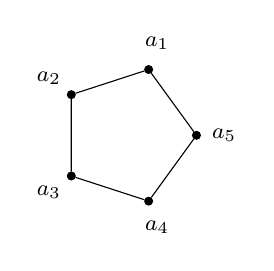
\begin{tikzpicture}
      \tikzstyle{node} = [draw,circle,fill=black,inner sep=1pt]
      \foreach \a in {1,2,...,5}{
        \draw (\a*360/5: 25pt) node(\a)[node]{};
        \draw (\a*360/5: 35pt) node{\footnotesize $a_\a$};
      }
      \path[draw] (1) -- (2) -- (3) -- (4) -- (5) -- (1);
    \end{tikzpicture}
    &
      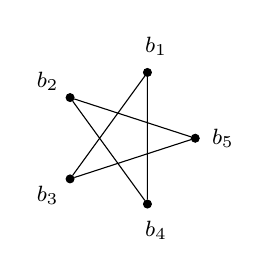
\begin{tikzpicture}
        \tikzstyle{node} = [draw,circle,fill=black,inner sep=1pt]
        \foreach \a in {1,2,...,5}{
          \draw (\a*360/5: 25pt) node(\a)[node]{};
          \draw (\a*360/5: 35pt) node{\footnotesize $b_\a$};
        }
        \path[draw] (2) -- (5) -- (3) -- (1) -- (4) -- (2);
      \end{tikzpicture}
    &
      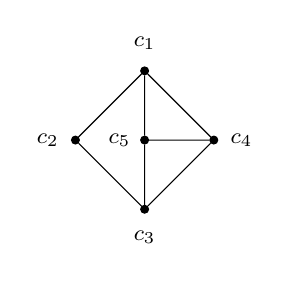
\begin{tikzpicture}
        \tikzstyle{node} = [draw,circle,fill=black,inner sep=1pt]
        \foreach \a in {1,2,...,4}{
          \draw (\a*360/4: 25pt) node(\a)[node]{};
          \draw (\a*360/4: 35pt) node{\footnotesize $c_\a$};
        }
        \node [node, label = left:\footnotesize $c_5$] (5) at (0,0) {};
        \path[draw] (1) -- (2) -- (3) -- (4) -- (1) -- (5) -- (4) -- (3) -- (5);
      \end{tikzpicture}
    &
      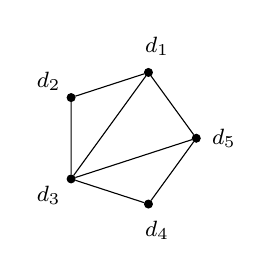
\begin{tikzpicture}
        \tikzstyle{node} = [draw,circle,fill=black,inner sep=1pt]
        \foreach \a in {1,2,...,5}{
          \draw (\a*360/5: 25pt) node(\a)[node]{};
          \draw (\a*360/5: 35pt) node{\footnotesize $d_\a$};
        }
        \path[draw] (1) -- (2) -- (3) -- (4) -- (5) -- (1) -- (3) -- (5);
      \end{tikzpicture}\\
    Graph A & Graph B & Graph C & Graph D    
  \end{tabular}    

  \begin{parts}
  \part[5] Graph A and Graph B
    \begin{solution}
      \textbf{Step 1:}\\
    We have equal number of vertices in both graphs i.e. $|V_{A}|=|V_{B}|$\\
    \textbf{Step 2:}\\
	\begin{tabular}{ |c|c| } 
	 \hline
	 Graph A & Graph B \\ 
	 \hline
	 $deg(a_{1})=2$ & $deg(b_{1})=2$ \\ 
	 $deg(a_{2})=2$ & $deg(b_{2})=2$ \\ 
	 $deg(a_{3})=2$ & $deg(b_{3})=2$ \\ 
	 $deg(a_{4})=2$ & $deg(b_{4})=2$ \\ 
	 $deg(a_{5})=2$ & $deg(b_{5})=2$ \\ 
	 \hline
	\end{tabular}\\
	
    Occurrence of degrees for both graph is similar i.e $\{2,2,2,2,2\}$\\
    \textbf{Step 3:}\\
    Determining if the isomorphic pair exists:\\
    \begin{tabular}{ |c|c| } 
	 \hline
	 Injective mapping &  Degree of neighboring pairs\\ 
	 \hline
	 $f(a{1})=b{1}$ & $deg(a_{2})=deg(b_{3})=2$, $deg(a_{5})=deg(b_{4})=2$ \\ 
	 $f(a{2})=b{3}$ & $deg(a_{1})=deg(b_{1})=2$, $deg(a_{3})=deg(b_{5})=2$ \\
	 $f(a{3})=b{5}$ & $deg(a_{2})=deg(b_{2})=2$, $deg(a_{4})=deg(b_{3})=2$ \\ 
	 $f(a{4})=b{2}$ & $deg(a_{3})=deg(b_{4})=2$, $deg(a_{5})=deg(b_{5})=2$ \\
	 $f(a{5})=b{4}$ & $deg(a_{1})=deg(b_{1})=2$, $deg(a_{4})=deg(b_{2})=2$ \\
	 \hline
	\end{tabular}\\
    \textbf{Step 4:}\\
    We have the following mapping of vertex which identify that Graph A and Graph B are isomorphic:\\
    \begin{tabular}{ |c|c| } 
	 \hline
	 Graph A Vertex & Graph B Vertex \\ 
	 \hline
	 $a_{1}\rightarrow$ & $\leftarrow b_{1}$ \\ 
	 $a_{2}\rightarrow$ & $\leftarrow b_{3}$ \\ 
	 $a_{3}\rightarrow$ & $\leftarrow b_{5}$ \\ 
	 $a_{4}\rightarrow$ & $\leftarrow b_{2}$ \\ 
	 $a_{5}\rightarrow$ & $\leftarrow b_{4}$ \\ 
	 \hline
	\end{tabular}
    \end{solution}

  \part[5] Graph A and Graph C
    \begin{solution}
      \textbf{Step 1:}\\
    We have equal number of vertices in both graphs i.e. $|V_{A}|=|V_{C}|$\\
    \textbf{Step 2:}\\
	\begin{tabular}{ |c|c| } 
	 \hline
	 Graph A & Graph C \\ 
	 \hline
	 $deg(a_{1})=2$ & $deg(c_{1})=3$ \\ 
	 $deg(a_{2})=2$ & $deg(c_{2})=2$ \\ 
	 $deg(a_{3})=2$ & $deg(c_{3})=3$ \\ 
	 $deg(a_{4})=2$ & $deg(c_{4})=3$ \\ 
	 $deg(a_{5})=2$ & $deg(c_{5})=3$ \\ 
	 \hline
	\end{tabular}\\
	
    Occurrence of degrees for both graph is different i.e $\{2,2,2,2,2\}$ and $\{2,3,3,3,3\}$\\
    Hence Graph A and Graph C are not isomorphic.
    \end{solution}
    
  \part[5] Graph A and Graph D
    \begin{solution}
        \textbf{Step 1:}\\
          We have equal number of vertices in both graphs i.e. $|V_{A}|=|V_{D}|$\\
          \textbf{Step 2:}\\
        \begin{tabular}{ |c|c| } 
         \hline
         Graph A & Graph D \\ 
         \hline
         $deg(a_{1})=2$ & $deg(d_{1})=3$ \\ 
         $deg(a_{2})=2$ & $deg(d_{2})=2$ \\ 
         $deg(a_{3})=2$ & $deg(d_{3})=4$ \\ 
         $deg(a_{4})=2$ & $deg(d_{4})=2$ \\ 
         $deg(a_{5})=2$ & $deg(d_{5})=3$ \\ 
         \hline
        \end{tabular}\\
        
          Occurrence of degrees for both graph is different i.e $\{2,2,2,2,2\}$ and $\{2,2,3,3,4\}$\\
          Hence Graph A and Graph D are not isomorphic.
    \end{solution}
    
  \part[5] Graph B and Graph C
    \begin{solution}
      \textbf{Step 1:}\\
    We have equal number of vertices in both graphs i.e. $|V_{B}|=|V_{C}|$\\
    \textbf{Step 2:}\\
	\begin{tabular}{ |c|c| } 
	 \hline
	 Graph B & Graph C \\ 
	 \hline
	 $deg(b_{1})=2$ & $deg(c_{1})=3$ \\ 
	 $deg(b_{2})=2$ & $deg(c_{2})=2$ \\ 
	 $deg(b_{3})=2$ & $deg(c_{3})=3$ \\ 
	 $deg(b_{4})=2$ & $deg(c_{4})=3$ \\ 
	 $deg(b_{5})=2$ & $deg(c_{5})=3$ \\ 
	 \hline
	\end{tabular}\\
	
    Occurrence of degrees for both graph is different i.e $\{2,2,2,2,2\}$ and $\{2,3,3,3,3\}$\\
    Hence Graph B and Graph C are not isomorphic.
    \end{solution}
    
  \part[5] Graph B and Graph D
    \begin{solution}
      \textbf{Step 1:}\\
    We have equal number of vertices in both graphs i.e. $|V_{B}|=|V_{D}|$\\
    \textbf{Step 2:}\\
	\begin{tabular}{ |c|c| } 
	 \hline
	 Graph B & Graph D \\ 
	 \hline
	 $deg(b_{1})=2$ & $deg(d_{1})=3$ \\ 
	 $deg(b_{2})=2$ & $deg(d_{2})=2$ \\ 
	 $deg(b_{3})=2$ & $deg(d_{3})=4$ \\ 
	 $deg(b_{4})=2$ & $deg(d_{4})=2$ \\ 
	 $deg(b_{5})=2$ & $deg(d_{5})=3$ \\ 
	 \hline
	\end{tabular}\\
	
    Occurrence of degrees for both graph is different i.e $\{2,2,2,2,2\}$ and $\{2,2,3,3,4\}$\\
    Hence Graph B and Graph D are not isomorphic.
    \end{solution}
    
  \part[5] Graph C and Graph D
    \begin{solution}
      \textbf{Step 1:}\\
      We have equal number of vertices in both graphs i.e. $|V_{C}|=|V_{D}|$\\
      \textbf{Step 2:}\\
    \begin{tabular}{ |c|c| } 
     \hline
     Graph C & Graph D \\ 
     \hline
     $deg(c_{1})=3$ & $deg(d_{1})=3$ \\ 
     $deg(c_{2})=2$ & $deg(d_{2})=2$ \\ 
     $deg(c_{3})=3$ & $deg(d_{3})=4$ \\ 
     $deg(c_{4})=3$ & $deg(d_{4})=2$ \\ 
     $deg(c_{5})=3$ & $deg(d_{5})=3$ \\ 
     \hline
    \end{tabular}\\
    
      Occurrence of degrees for both graph is different i.e $\{2,3,3,3,3\}$ and $\{2,2,3,3,4\}$\\
      Hence Graph C and Graph D are not isomorphic.
      \end{solution}
  \end{parts}

\question[5] Show that in a simple graph with at least two vertices there must be two vertices that have the same degree.
  \begin{solution}\\
    Let's assume that a Graph $G(V,E)$ contain n vertices.\\
    Since, it has n vertices, then it is obvious that the possible degree can be $0,1,2,3, ... , n-1$.\\
    Nevertheless, it can be said that the Graph $G(V,E)$ cannot contain one vertex of degree $0$ and some other vertex of degree $n-1$ as these two vertices need to be adjacent to each other to satisfy degree n-1.\\
    By using the pigeonhole theorem, we must pick the $n$ degrees; one for each vertex from a set of $n-1$ answers; since we cannot have both $n-1$ and zero.\\
    Hence, one degree must be repeated which implies that there are two vertices with the same degree.\\
    \textbf{Note:}\\
    It is not true for Graphs with no loops.\\
    It is not true for Graphs with multiple edges.\\
  \end{solution}
  
\question[5] The \textit{complementary graph} $\overline{G}$ of a simple graph $G$ has the same vertices as  $G$. Two vertices are adjacent in $\overline{G}$ if and only if they are not adjacent in $G$. Given $G$ with $v$ vertices and $e$ edges, how many edges are there in $\overline{G}$? Justify your answer.
  \begin{solution}
    Since we have a simple graph $G$, that mean we have no multiple edges or loops for different vertices. And considering we have $e$ edges for $G$ and $\bar{e}$ edges for $\bar{G}$, then the sum $e+e'$ should contain all the possible edges for each vertex in a simple graph that is $v-1$ edges for each vertex which is the case for a complete simple graph.\\
	We also know that total edges for a complete graph with $n$ vertices is $\frac{n(n-1)}{2}$.\\
	Hence by the above statement, we should have the following edges for the complementary graph:
	\begin{center}
	$Edges\  of\  \bar{G}=E(\bar{G})=\frac{v(v-1)}{2} - e$
	\end{center}
  \end{solution}
  
  \section*{Induction}
  
\question Prove the following using induction.
  \begin{parts}
  \part[5] Given a a relation $R$ that is reflexive and transitive, $R^n = R$ for all positive integers $n$.
    \begin{solution}\\
      % Write your solution here
      \textbf{Given:}\\
      Relation $R$ on a set $X$ is transitive and reflexive.\\
      \textbf{To Prove:}\\
      For all positive integers n, $R^n = R$ holds.\\
      \textbf{Proof by Induction:}\\
      Let the statement $R^n = R$ be $P(n)$.\\
      \textbf{Base Case (n = 1):}\\
      The result is true because $R = R$ is always true and $R^1 = R$.\\
      \textbf{Inductive Case:}\\
      Assuming, $P(n)$ is true.\\
      $R^n = R$\\
      then we need to prove that $P(n + 1)$ is also true.\\
      $R^{n+1} = R^n . R$\\
      $R^{n+1} = R . R$\\
      Let $(a,b) \in R$.\\
      Since, R is reflexive then $(b,b) \in R$.\\
      According to definition of composition, $(a,b) \in R . R = R^{n+1}$\\
      $R \subseteq R^{n+1}$
      Now,
      Let, $(a,b) \in R^{n+1} = R . R$\\
      By composite property:\\
      $\exists c \in R: (a,c) \in R and (c,b) \in R$\\
      By transitive property:\\
      $R^{n+1} \subseteq R$\\
      Since $R^{n+1} \subseteq R$ and $R \subseteq R^{n+1}$, we have then shown:\\
      $R^{n+1} = R$\\
      Thus;\\
      $P(n+1)$ is true.\\
      Hence, by the principle of mathematical induction, $P(n)$ is true for all positive integers n.
    \end{solution}

  \part[5] A relation $R$ on a set $A$ is transitive if and only if $R^n \subseteq R$ for all positive integers $n$.
    \begin{solution}\\
      % Write your solution here
      \textbf{Given:}\\
      Relation $R$ on a set $A$ is transitive.\\
      \textbf{To Prove:}\\
      $R^n \subseteq R$, for all positive integers n.\\
      \textbf{Proof by Induction:}\\
      The Result is trivially true for n = 1.\\
      Assuming, $R^n \subseteq R$ for some $n \geq 1$.\\
      Let, $(x,y) \in R^{n+1}$.\\
      Since, $R^{n+1} = R^n . R$, there exists an element $z \in A$ such that $(x,z) \in R^n$ and $(z,y) \in R$.\\
      Then According to Inductive Hypothesis:\\
      $R^n \subseteq R$ implies that $(x,z) \in R$.\\
      Since, R is transitive then $(x,z) \in R$ and $(z,y) \in R$ imply that $(x,y) \in R$.\\
      thus,\\
      $R^{n+1} = R$ is proved by the mathematical induction.
    \end{solution}
  \end{parts}


\question[5] Prove via induction that a complete graph with $n$ vertices contains $\dfrac{n(n-1)}{2}$ edges.
  \begin{solution}
    In complete graph with $n$ vertices, each vertex contains $(n-1)$ vertex and we have total vertices given by following summation:
	\[
    \sum_{i=1}^{n} (n-i) = (n-1)+(n-2)+(n-3) ... +3+2+1 = \dfrac{n(n-1)}{2}
  \]\\
    \textbf{Proof}\\
    \textbf{Base Step:}\\
    Let n=1, then we have,\\
	$(1-1)=\dfrac{1(1-1)}{2}$\\
	$0=\dfrac{1(0)}{2}$\\
	$0=0$\
  Hence, this is true.\
	\textbf{Induction Step:}\\
	Now lets assume above expression is true for $n=k$, that is the following expression is true,
    \begin{center}
    $(k-1)+(k-2)+(k-3) ... +3+2+1 = \dfrac{k(k-1)}{2}$
    \end{center}
  Now lets assume $n=k+1$, for which we would have,\\
  $((k+1)-1)+((k+1)-2)+((k+1)-3) ... +3+2+1 = \dfrac{(k+1)((k+1)-1)}{2}$\\
  To prove above statement we have,\\
  RHS:\\ 
  $=\dfrac{(k+1)((k+1)-1)}{2}$\\
  $=\dfrac{(k+1)(k)}{2}$\\
  $=\dfrac{(k^{2}+k)}{2}$\\
  
  LHS:\\
    $=((k+1)-1)+((k+1)-2)+((k+1)-3) ... +3+2+1$\\
    $=(k)+(k-1)+(k-2) ... +3+2+1$\\
    But from above, we have assumed the following:\\
    $(k-1)+(k-2)+(k-3) ... +3+2+1 = \dfrac{k(k-1)}{2}$\\
    Hence substituting it in the previous expression, we would get:\\
    $=(k)+\dfrac{k(k-1)}{2}$\\
    $=\dfrac{2k+k(k-1)}{2}$\\
    $=\dfrac{2k+k^{2}-k}{2}$\\
    $=\dfrac{k^{2}+k}{2}$\\
    
    Hence we have LHS=RHS proved via induction.
  \end{solution}
  
\end{questions}
\end{document}


%%% Local Variables:
%%% mode: latex
%%% TeX-master: t
%%% End:
